% vim:ft=tex:
%
\documentclass[8pt]{beamer}

\usepackage{times}
\usepackage{graphicx}
\usepackage[]{geometry}
\usepackage{booktabs}
\usepackage{hyperref}
\usepackage{pdfpages}
\usepackage{enumitem}

\usetheme{Montpellier}
\usecolortheme{beaver}
\setbeamertemplate{navigation symbols}{}

\usepackage{xcolor}

\definecolor{asparagus}{rgb}{0.53, 0.66, 0.42}
\definecolor{aurometalsaurus}{rgb}{0.43, 0.5, 0.5}
\definecolor{beige}{rgb}{0.96, 0.96, 0.86}
\setbeamercolor{titlelike}{parent=palette primary,fg=asparagus}
\setbeamercolor*{palette primary}{bg=beige, fg=asparagus}
\setbeamercolor*{palette secondary}{bg=beige!90!aurometalsaurus, fg=asparagus}
\setbeamercolor*{palette tertiary}{bg=aurometalsaurus, fg=asparagus}
\setbeamercolor*{palette quaternary}{bg=beige, fg=asparagus}
\setbeamercolor{frametitle}{bg=aurometalsaurus!10!beige}
\setbeamercolor{frametitle right}{bg=aurometalsaurus!60!beige}
\setbeamertemplate{itemize item}{\color{asparagus}$\blacktriangleright$}

\hypersetup{colorlinks,urlcolor=asparagus}

\setlist[itemize]{itemsep=10pt, label={\color{asparagus}$\blacktriangleright$}}

\usepackage{tikz}
% \usetikzlibrary{positioning, decorations.pathmorphing, shapes}

\newcommand{\positionone}{\textbf{Position n}}
\newcommand{\positiontwo}{\textbf{Position n + i }}
\newcommand{\yslant}{0.5}
\newcommand{\xslant}{-0.6}
\newcommand{\yslantHori}{0.55}
\newcommand{\xslantHori}{0.0}

% \usetikzlibrary{shapes.geometric,arrows.meta}
\usepackage[edges]{forest}
\usepackage{adjustbox}
\usepackage{float}
\usepackage{graphicx}
\usepackage{booktabs}

\usetikzlibrary{positioning, decorations.pathmorphing, shapes, shapes.geometric,arrows.meta}

\title{DNA analysis in population genetics\\
Practical 3, Summary statistics and Linkage Disequilibrium}

\date{March, 9, 2020}

\author{
    \texorpdfstring{
        \begin{columns}
              \column{.45\linewidth}
              \centering
              Chedly Kastally\\
              \href{mailto:chedly.kastally@oulu.fi}{chedly.kastally@oulu.fi}
              \column{.45\linewidth}
              \centering
              Tanja Pyh{\"a}j{\"a}rvi\\
              \href{mailto:tanja.pyhajarvi@oulu.fi}{tanja.pyhajarvi@oulu.fi}
        \end{columns}
    % \texorpdfstring{}
    }
    {Kastally, Chedly \and Tanja Pyh{\"a}j{\"a}rvi}
}

\begin{document}

\begin{frame}
\titlepage
\end{frame}

\forestset{
leftstrike/.style={
  edge label={
      node[midway, xshift=7mm, red, yshift=0mm, rotate=90] {---}
  }
},
rightstrike/.style={
  edge label={
      node[midway, xshift=-7mm, red, yshift=0mm, rotate=90] {---}
  }
}
}

\begin{frame}
    \frametitle{About R}

    \begin{minipage}{.6\textwidth}
    \begin{itemize}
    
        \item<1-> Some resources for R: ``R for Data Science'' by Garrett
            Grolemund and Hadley Wickham. Free \& open version available online.

            \url{https://r4ds.had.co.nz/index.html}.

        \item<2-> Use Integrated Development Environment to code. There
            are plenty of options in R, notably,
            \href{https://rstudio.com/}{Rstudio} or
            \href{https://nbcgib.uesc.br/tinnr/en/}{Tinn-R}.
            Choose one, and master it, to produce R code
            efficiently.

    \end{itemize}
\end{minipage}%
    \begin{minipage}{.3\textwidth}
        \flushright
            \onslide<1->{\includegraphics[width=0.7\textwidth]{cover.png}}
\end{minipage}

\end{frame}

\begin{frame}
    \frametitle{Demographic processes}

    \large

    \begin{itemize}
    
        \item<1-> In population genetics, we are interested in understanding how
            various processes, such as demographic processes, impact genetic
            variation.

        \item<2-> As we have seen previously, we can use models, such as
            the \textit{coalescent}, to understand how various processes
            work and impact the biodiversity

        \item<3-> Today we will focus on analyzing data as if it were
            collected and given for you to analyze.

    \end{itemize}

\end{frame}

\begin{frame}
    \frametitle{Reminder note on the four gametes test}

    \small
    \onslide<1->4 DNA fragments, we assign two mutations (IFS model).

    \small
    \centering{}

\begin{adjustbox}{max height=.6\textheight}
\begin{tikzpicture}[
    scale=0.6,
    every node/.style={minimum size=0.5cm},
    on grid,
    decoration={coil},
    dna/.style={decorate, thick, decoration={aspect=0, segment length=0.35cm}}]


        % 2 vertical lines for linking agents on the 2 levels
        % \draw[dna](0.65,10.0) -- (0.65,0.6);
        % \draw[dna](0.65,9.9) -- (0.65,0.6);

        \onslide<1->\draw[dna](5.7,-2.3) -- (-0.1,3.6);
        \onslide<1->\draw[dna](5.6,-2.2) -- (-0.0,3.5);

        \onslide<1->\draw[dna](7.8,-1.2) -- (2.0,4.6);
        \onslide<1->\draw[dna](7.7,-1.1) -- (2.0,4.6);

        \onslide<1->\draw[dna](9.8,-0.1) -- (4.1,5.6);
        \onslide<1->\draw[dna](9.7,-0.0) -- (4.1,5.6);

        \onslide<1->\draw[dna](11.9,0.9) -- (6.2,6.6);
        \onslide<1->\draw[dna](11.8,1.0) -- (6.2,6.6);

        % Position n
        \onslide<2->\begin{scope}[
                xshift=0,
                yshift=0,
                every node/.append style={yslant=\yslantHori,xslant=\xslantHori},
                yslant=\yslantHori,xslant=\xslantHori
        ]

                % The frame:
                \onslide<2->\fill[white,fill opacity=.75] (0,2) rectangle (8,6); % Opacity
                \onslide<2->\draw[black, dashed, thin]    (0,1) rectangle (8,6);

                % The coalescent
                \onslide<2->\draw[thin]
                    (4,5.5) -- (4,5)     % hori
                    (4,5) -- (2.1,5)     % hori
                    (2.1,5) -- (2.1,3)   % vert
                    (4,5) -- (6.1,5)
                    (6.1,5) -- (6.1,3);

                \onslide<2->\draw[thin]
                        (1.9,3) -- (1,3) % Labour Powers
                        (1,3) -- (1,2)   % Labour Powers
                        (1.9,3) -- (3,3) % Labour Powers
                        (3,3) -- (3,2);  % Labour Powers

                \onslide<2->\draw[thin]
                        (5.9,3) -- (5,3) % Labour Powers
                        (5,3) -- (5,2)   % Labour Powers
                        (5.9,3) -- (7,3) % Labour Powers
                        (7,3) -- (7,2);  % Labour Powers

                % end nodes ;
                \onslide<2->\draw[fill=black]
                        (1,2) circle (.15) % A
                        (3,2) circle (.15); % A

                \onslide<2->{\fill[black]
                (0.2,5.5) node[right, scale=.7]{\positionone};}

                \only<2,3>\draw[fill=black]
                        (5,2) circle (.15) % B
                        (7,2) circle (.15); % B

                \only<4>\draw[red]
                        (5.9,4.6) -- (6.3,4.6); % mutation

                \only<4>\draw[fill=red]
                        (5,2) circle (.15) % B
                        (7,2) circle (.15); % B

                \only<4>\fill[black]
                        (1.1,1.6) node[left,scale=.7]{\textbf{A}}
                        (3.1,1.6) node[left,scale=.7]{\textbf{A}}
                        (5.1,1.6) node[left,scale=.7]{\textbf{B}}
                        (7.1,1.6) node[left,scale=.7]{\textbf{B}};
        \end{scope}

        % Position n + i
        \onslide<3->\begin{scope}[
                xshift=100,
                yshift=-100,
                every node/.append style={yslant=\yslantHori,xslant=\xslantHori},
                yslant=\yslantHori,xslant=\xslantHori
        ]

                % The frame:
                \onslide<3->\fill[white,fill opacity=.75] (0,1.85) rectangle (8,6); % Opacity
                \onslide<3->\draw[black, dashed, thin]    (0,1) rectangle (8,6);

                % the coalescent
                \onslide<3->\draw[thin]
                    (4,5.5) -- (4,5) % hori
                    (4,5) -- (2.1,5) % hori
                    (2.1,5) -- (2.1,3) % vert
                    (4,5) -- (6.1,5)
                    (6.1,5) -- (6.1,3);

                \onslide<3->\draw[thin]
                        (1.9,3) -- (1,3) % Labour Powers
                        (1,3) -- (1,2)   % Labour Powers
                        (1.9,3) -- (3,3) % Labour Powers
                        (3,3) -- (3,2);  % Labour Powers

                \onslide<3->\draw[thin]
                        (5.9,3) -- (5,3) % Labour Powers
                        (5,3) -- (5,2)   % Labour Powers
                        (5.9,3) -- (7,3) % Labour Powers
                        (7,3) -- (7,2);  % Labour Powers

                % end nodes
                        \only<3>{\draw[fill=black] (3,2) circle (.15);} % A

                \onslide<3->\draw[fill=black]
                        (1,2) circle (.15)  % A
                        (5,2) circle (.15)  % B
                        (7,2) circle (.15); % B

                \onslide<3->\fill[black]
                        (0.2,5.5) node[right, scale=.7] {\positiontwo};

                \only<4>\draw[fill=red]
                        (3,2) circle (.15); % A

                \only<4>\draw[thin,red]
                        (2.8,2.5) -- (3.15,2.5); % mutation

                \only<4>\fill[black]
                        (1.1,1.6) node[left,scale=.7]{\textbf{A}}
                        (3.1,1.6) node[left,scale=.7]{\textbf{B}}
                        (5.1,1.6) node[left,scale=.7]{\textbf{A}}
                        (7.1,1.6) node[left,scale=.7]{\textbf{A}};
        \end{scope}

\end{tikzpicture}

\end{adjustbox}

\flushleft{}

\small

\onslide<3->{Close positions share the same history, i.e.\ the same genealogy.}

\onslide<4->{Mutations are thrown randomly on each coalescent}

\end{frame}

\begin{frame}
    \frametitle{The four gamete tests, other combinations}

    \onslide<1-> As mutations are random, we can expect other possible
    combinations of mutations.
    

\begin{table}[ht]
\begin{minipage}{0.47\textwidth}
\centering{}
\begin{adjustbox}{max width=.8\textwidth}
\onslide<1->\begin{forest}
    forked edges,
    before typesetting nodes={%
        delay={%
            where content={}{coordinate}{},
        },
    },
    for tree={%
        grow'=0,
        s sep'+=5pt,
        l sep'+=25pt,
    },
    l sep'+=10pt,
  [
  [
  [A]
  [A]
  ]
  [, leftstrike
  [B, red]
  [B, red]
  ]
  ]
\end{forest}
\begin{forest}
    forked edges,
    before typesetting nodes={%
        delay={%
            where content={}{coordinate}{},
        },
    },
    for tree={%
        grow'=180,
        s sep'+=5pt,
        l sep'+=25pt,
    },
  l sep'+=10pt,
  [
  [
  [A]
  [A]
  ]
  [, rightstrike
  [B, red]
  [B, red]
  ]
  ]
\end{forest}

\end{adjustbox}
\begin{adjustbox}{max width=.5\textwidth}
\begin{tabular}{l | c c c c}
    Genotypes & AA & AB & BB & BA \\
    \midrule
    count & 0 & 2 & 0 & 2 \\
    \end{tabular}
\end{adjustbox}

\begin{adjustbox}{max width=.8\textwidth}
\onslide<2->\begin{forest}
    forked edges,
    before typesetting nodes={%
        delay={%
            where content={}{coordinate}{},
        },
    },
    for tree={%
        grow'=0,
        s sep'+=5pt,
        l sep'+=25pt,
    },
    l sep'+=10pt,
  [
  [, leftstrike
  [B, red]
  [B, red]
  ]
  [
  [A]
  [A]
  ]
  ]
\end{forest}
\begin{forest}
    forked edges,
    before typesetting nodes={%
        delay={%
            where content={}{coordinate}{},
        },
    },
    for tree={%
        grow'=180,
        s sep'+=5pt,
        l sep'+=25pt,
    },
  l sep'+=10pt,
  [
  [
  [A]
  [A]
  ]
  [, rightstrike
  [B, red]
  [B, red]
  ]
  ]
\end{forest}

\end{adjustbox}
\begin{adjustbox}{max width=.5\textwidth}
\begin{tabular}{l | *4{c}}
    \onslide<2->{Genotypes & AA & AB & BB & BA}%
    \onslide<2->{\\\midrule}
    \onslide<2->{count & 2 & 0 & 2 & 0}  \\
\end{tabular}
\end{adjustbox}
\end{minipage}%
\begin{minipage}{0.47\textwidth}
\centering{}
\begin{adjustbox}{max width=.8\textwidth}
\onslide<3->{\begin{forest}
    forked edges,
    before typesetting nodes={%
        delay={%
            where content={}{coordinate}{},
        },
    },
    for tree={%
        grow'=0,
        s sep'+=5pt,
        l sep'+=25pt,
    },
    l sep'+=10pt,
  [
  [
  [B, red, leftstrike]
  [A]
  ]
  [
  [A]
  [A]
  ]
  ]
\end{forest}
\begin{forest}
    forked edges,
    before typesetting nodes={%
        delay={%
            where content={}{coordinate}{},
        },
    },
    for tree={%
        grow'=180,
        s sep'+=5pt,
        l sep'+=25pt,
    },
  l sep'+=10pt,
  [
  [
  [A]
  [A]
  ]
  [, rightstrike
  [B, red]
  [B, red]
  ]
  ]
\end{forest}}

\end{adjustbox}
\begin{adjustbox}{max width=.5\textwidth}
\begin{tabular}{l | c c c c}
    \onslide<3->{Genotypes & AA & AB & BB & BA}
    \onslide<3->{\\\midrule}
    \onslide<3->{count & 2 & 1 & 1 & 0} \\
\end{tabular}
\end{adjustbox}

\begin{adjustbox}{max width=.8\textwidth}
\onslide<4->{\begin{forest}
    forked edges,
    before typesetting nodes={%
        delay={%
            where content={}{coordinate}{},
        },
    },
    for tree={%
        grow'=0,
        s sep'+=5pt,
        l sep'+=25pt,
    },
    l sep'+=10pt,
  [
  [
  [A]
  [A]
  ]
  [
  [B, red, leftstrike]
  [A]
  ]
  ]
\end{forest}
\begin{forest}
    forked edges,
    before typesetting nodes={%
        delay={%
            where content={}{coordinate}{},
        },
    },
    for tree={%
        grow'=180,
        s sep'+=5pt,
        l sep'+=25pt,
    },
  l sep'+=10pt,
  [
  [
  [A]
  [A]
  ]
  [, rightstrike
  [B, red]
  [B, red]
  ]
  ]
\end{forest}}

\end{adjustbox}
\begin{adjustbox}{max width=.5\textwidth}
\begin{tabular}{l | c c c c}
    \onslide<4->{Genotypes & AA & AB & BB & BA}
    \onslide<4->{\\\midrule}
    \onslide<4->{count & 1 & 2 & 0 & 1} \\
    \end{tabular}
\end{adjustbox}

\end{minipage}
\end{table}

\small 
\onslide<5-> Similar variations are possible, but no matter where you
put the two mutations, you always have a maximum of three genotypes for
a given configuration

\end{frame}

\begin{frame}
    \frametitle{The four gamete tests, conclusion}

    \onslide<1-> How could we explain a case with 4 genotypes if we
    observe such cases?

\begin{table}[ht]
\begin{minipage}{0.47\textwidth}
\centering{}
\begin{adjustbox}{max width=.8\textwidth}
\onslide<2->\begin{forest}
    forked edges,
    % /tikz/every pin edge/.append style={Latex-, shorten <=2.5pt, darkgray},
    % /tikz/every pin/.append style={darkgray, font=\sffamily},
    % /tikz/every label/.append style={darkgray, font=\sffamily},
    before typesetting nodes={
        delay={
            where content={}{coordinate}{},
        },
        % where n children=0{tier=terminus, label/.process={Ow{content}{right:#1}}, content=}{},
    },
    for tree={
        grow'=0,
        s sep'+=5pt,
        l sep'+=25pt,
    },
  l sep'+=10pt,
  [,
    [
      % [
        [A]
      % ]
      [A]
    ]
    [,leftstrike
    [B, red][B, red]]
  ]
\end{forest}%
\begin{forest}
    forked edges,
    % /tikz/every pin edge/.append style={Latex-, shorten <=2.5pt, darkgray},
    % /tikz/every pin/.append style={darkgray, font=\sffamily},
    % /tikz/every label/.append style={darkgray, font=\sffamily},
    before typesetting nodes={
        delay={
            where content={}{coordinate}{},
        },
        % where n children=0{tier=terminus, label/.process={Ow{content}{left:#1}}, content=}{},
    },
    for tree={
        grow'=180,
        s sep'+=5pt,
        l sep'+=10pt,
    },
  l sep'+=2pt,
  [
    [
            [A, tier=final]
        [, rightstrike
            [B, red, tier=final]
            [B, red, tier=final]
        ]
    ]
            [A, tier=final]
  ]
\end{forest}
\end{adjustbox}
\begin{adjustbox}{max width=.5\textwidth}
\begin{tabular}{l | c c c c}
    \onslide<2->{Genotypes & AA & AB & BB & BA}
    \onslide<2->{\\\midrule}
    \onslide<2->{count & 1 & 1 & 1 & 1} \\
    \end{tabular}
\end{adjustbox}

\vspace{2pt}
\onslide<2->{\flushleft\tiny{A \textit{recombination} event (a change in the genealogie of one locus)
might produce such pattern.}}

\end{minipage}%
\begin{minipage}{0.47\textwidth}
\centering{}
\begin{adjustbox}{max width=.8\textwidth}
\onslide<3->{\begin{forest}
    forked edges,
    before typesetting nodes={%
        delay={%
            where content={}{coordinate}{},
        },
    },
    for tree={%
        grow'=0,
        s sep'+=5pt,
        l sep'+=25pt,
    },
    l sep'+=10pt,
  [
  [
  [A]
  [B, red, leftstrike]
  ]
  [
  [B, red, leftstrike]
  [A]
  ]
  ]
\end{forest}
\begin{forest}
    forked edges,
    before typesetting nodes={%
        delay={%
            where content={}{coordinate}{},
        },
    },
    for tree={%
        grow'=180,
        s sep'+=5pt,
        l sep'+=25pt,
    },
  l sep'+=10pt,
  [
  [
  [A]
  [A]
  ]
  [, rightstrike
  [B, red]
  [B, red]
  ]
  ]
\end{forest}}
\end{adjustbox}
\begin{adjustbox}{max width=.5\textwidth}
\begin{tabular}{l | c c c c}
    \onslide<3->{Genotypes & AA & AB & BB & BA}
    \onslide<3->{\\\midrule}
    \onslide<3->{count & 1 & 1 & 1 & 1} \\
    \end{tabular}
\end{adjustbox}

\vspace{3pt}
\onslide<3->{\tiny{A second mutation might produce such pattern.}}

\end{minipage}
\end{table}

\begin{itemize}

    \item<4->When we assume the IFS mutation model (only one mutation
        per coalescent), we can deduce there has a been a recombination event
        between the two polymorphic sites.

    \item<5->When the mutation rate $\mu$ is much higher that the recombination
        rate $c$, this is a reasonable conclusion. This is not the case if the
        organism of interest has a very low recombination rate.

    \item<6->Note, however, that not all recombination events will be
        detected with a FGT\@.

\end{itemize}

\end{frame}

\begin{frame}
    \frametitle{Goals of today's session}

    \begin{itemize}
    
        \item Practice reading and manipulating genetic data with R (fasta and vcf files)

    \item Compute and plot summary statistics:
        \begin{itemize}
            \setlength\itemsep{2pt}
        
            \item compute and plot the (folded and unfolded) site frequency spectrum
            \item compute and plot the expected site frequency spectrum
            \item compute Tajima's D and $\pi$
            \item compute Linkage disequilibrium related statistics: D' and $r^2$
        
        \end{itemize}

    \item Observe the trace of linkage disequilibrium in sequences
        \begin{itemize}
            \setlength\itemsep{2pt}
            \item Perform the 4 gametes test on a set of sequences
            \item infer the minimum number of recombination events
        \end{itemize}

    \item If you have the time,
        \begin{itemize}
            \setlength\itemsep{2pt}
            \item model $r^2$ decay across contigs
            \item linkage mapping using $r^2$
        \end{itemize}

    \end{itemize}

\end{frame}

\end{document}

% vertical alternative
% \begin{tikzpicture}[
%     scale=0.6,
%     every node/.style={minimum size=.3cm},
%     on grid,
%     decoration={coil},
%     dna/.style={decorate, thick, decoration={aspect=0, segment length=0.5cm}}]
%
%
%         % 2 vertical lines for linking agents on the 2 levels
%         % \draw[dna](0.65,10.0) -- (0.65,0.6);
%         % \draw[dna](0.65,9.9) -- (0.65,0.6);
%
%         \draw[dna](-0.2,4.0) -- (-0.2,-4.6);
%         \draw[dna](-0.2,4.1) -- (-0.2,-4.6);
%         \draw[dna](1.8,5.0) -- (1.8,-3.6);
%         \draw[dna](1.8,5.1) -- (1.8,-3.6);
%         \draw[dna](3.8,6.0) -- (3.8,-2.6);
%         \draw[dna](3.8,6.1) -- (3.8,-2.6);
%         \draw[dna](5.8,7.0) -- (5.8,-1.6);
%         \draw[dna](5.8,7.1) -- (5.8,-1.6);
%
%
%         % Real level
%         \begin{scope}[
%                 yshift=-130,
%                 every node/.append style={yslant=\yslant,xslant=\xslant},
%                 yslant=\yslant,xslant=\xslant
%         ]
%
%                 % The frame:
%                 \fill[white,fill opacity=.75] (0,0) rectangle (8,2); % Opacity
%                 \draw[black, dashed, thin]    (0,0) rectangle (9,6);
%                 % Agents:
%                 \draw[fill=black]
%                         (1,2) circle (.1) % A
%                         (3,2) circle (.1); % A
%                 \draw[fill=red]
%                         (5,2) circle (.1) % B
%                         (7,2) circle (.1); % B
%                 % Flows:
%                 \draw[thin]
%                     (4,5.5) -- (4,5) % hori
%                     (4,5) -- (2.1,5) % hori
%                     (2.1,5) -- (2.1,3) % vert
%                     (4,5) -- (6.1,5)
%                     (6.1,5) -- (6.1,3);
%                 \draw[thin]
%                         (1.9,3) -- (1,3) % Labour Powers
%                         (1,3) -- (1,2) % Labour Powers
%                         (1.9,3) -- (3,3) % Labour Powers
%                         (3,3) -- (3,2); % Labour Powers
%                     %
%                 \draw[thin]
%                         (5.9,3) -- (5,3) % Labour Powers
%                         (5,3) -- (5,2)% Labour Powers
%                         (5.9,3) -- (7,3) % Labour Powers
%                         (7,3) -- (7,2); % Labour Powers
%                 \draw[line width=1.3pt,red]  % mutation
%                         (5.9,3.2) -- (6.3,3.2); % mutation
%                  % Labels:
%                 \fill[black]
%                         (0.5,6.5) node[right, scale=.7] {\positionone}
%                         (1.3,1.5) node[left,scale=.7]{\textbf{A}}
%                         (3.3,1.5) node[left,scale=.7]{\textbf{A}}
%                         (5.3,1.5) node[left,scale=.7]{\textbf{B}}
%                         (7.3,1.5) node[left,scale=.7]{\textbf{B}};
%         \end{scope}
%
%         \begin{scope}[
%                 yshift=0,
%                 every node/.append style={yslant=\yslant,xslant=\xslant},
%                 yslant=\yslant,xslant=\xslant
%         ]
%
%                 % The frame:
%                 \fill[white,fill opacity=.75] (0,0) rectangle (8,2); % Opacity
%                 \draw[black, dashed, thin]    (0,0) rectangle (8,6);
%                 % % The frame:
%                 % \draw[black, dashed, thin] (0,0) rectangle (9,9);
%                 % Agents:
%                 \draw[fill=black]
%                         (1,2) circle (.1) % A
%                         (5,2) circle (.1) % B
%                         (7,2) circle (.1); % B
%                 \draw[fill=red]
%                         (3,2) circle (.1); % A
%                 % Flows:
%                 \draw[thin]
%                     (4,5.5) -- (4,5) % hori
%                     (4,5) -- (2.1,5) % hori
%                     (2.1,5) -- (2.1,3) % vert
%                     (4,5) -- (6.1,5)
%                     (6.1,5) -- (6.1,3);
%                 \draw[thin]
%                         (1.9,3) -- (1,3) % Labour Powers
%                         (1,3) -- (1,2) % Labour Powers
%                         (1.9,3) -- (3,3) % Labour Powers
%                         (3,3) -- (3,2); % Labour Powers
%                     %
%                 \draw[thin]
%                         (5.9,3) -- (5,3) % Labour Powers
%                         (5,3) -- (5,2)% Labour Powers
%                         (5.9,3) -- (7,3) % Labour Powers
%                         (7,3) -- (7,2); % Labour Powers
%                 \draw[line width=1.3pt,red]  % mutation
%                         (2.8,2.5) -- (3.15,2.5); % mutation
%                  % Labels:
%                 \fill[black]
%                         (0.5,6.5) node[right, scale=.7] {\positiontwo}
%                         (1.3,1.5) node[left,scale=.7]{\textbf{A}}
%                         (3.3,1.5) node[left,scale=.7]{\textbf{B}}
%                         (5.3,1.5) node[left,scale=.7]{\textbf{A}}
%                         (7.3,1.5) node[left,scale=.7]{\textbf{A}};
%         \end{scope}
% \end{tikzpicture}

